   
        \section{Overview of multivariate functions}
        Aside from the study of linear transformations on $\R^n$ or $\C^n$, we have limited ourselves to functions of a single variable.  Given that we have performed a deep analysis for functions of one variable, we can take what we have learned and apply it to new types of functions. Specifically, we will concentrate on $\R^3$ (or $\R^2$) and functions of the form:
        \begin{align*}
            &\curvegamma\colon \R \to \R^3\\
            &f\colon \R^3 \to \R\\
            &\vecfieldV \colon \R^3 \to \R^3.
        \end{align*}
        Of these three functions, the latter two are often referred to as \boldgreen{fields}.  These are also \boldgreen{multivariate} functions, whereas the first only has an input of a single variable.
        
        
        \begin{enumerate}[(1)]
        \item Functions of the form
        \[
        \curvegamma \colon \R\to \R^3
        \]
        are \boldgreen{curves}.  Often times, we will have 
        \[
        \curvegamma \colon [a,b]\to \R^3
        \]
        when we want curves with specific endpoints. We will concentrate first on curves, so I'll save the extra detail for a bit later.
        
        \item Functions of the form
        \[
        f\colon \R^3 \to \R
        \]
        are \boldgreen{scalar fields} .   These functions are useful in describing quantities like temperature in space.  In this example, at each point $\vecx$ in space $\R^3$, we can assign a single real number output $f(\vecx)$ that tells us this temperature.  
        
        %One may ask how this function changes from point to point.  Asking this question sends you immediately to investigating the \emph{gradient}.  It turns out, using our temperature example, that we can understand heat flow by understanding temperature gradients.
        
        \item Functions of the form
        \[
        \vecfieldV \colon \R^3 \to \R^3
        \]
        are called \boldgreen{vector fields}.  Roughly speaking, at each point $\vecx$ in space $\R^3$, we can place a vector $\vecfieldV(\vecx)$ that is also in $\R^3$.  These fields are very important in describing systems that have flow.  For example, fluid flow or electromagnetism are vector field theories. 
        
        % What will it mean to find the change in a vector field?  This will lead us to the notion of the \emph{total derivative}.  This concept is a bit abstract at first but will really tell us the proper notion of the derivative.
        \end{enumerate}
        
        
        \section{Curves in space}
        
        We will begin with curves as they are very useful tools and this will help us visualize results for the other types of functions. 
        
        Let us consider a curve
        \[
        \curvegamma \colon \R \to \R^3.
        \]
        We will specify a specific curve by supplying three functions $f_1(t)$, $f_2(t)$, and $f_3(t)$. Specifically, each of these functions $f_i$ is a function $f_i\colon \R \to \R$. Then, we can say that
        \[
        \curvegamma(t)=\begin{pmatrix} \gamma_1(t)\\ \gamma_2(t)\\ \gamma_3(t)\end{pmatrix}.
        \]
       Each $\gamma_i(t)$ (for the values $i=1,2,3$) represents the components of a vector that changes with respect to the variable $t$. Intuitively, we like to think of the components as evolving in time, which is why we make use of the variable $t$. To say this more explicitly, we can write
        \begin{align*}
            &\gamma_1(t) \quad \textrm{the $x$-position of $\gamma$ at time $t$,}\\
            &\gamma_2(t) \quad \textrm{the $y$-position of $\gamma$ at time $t$,}\\
            &\gamma_3(t) \quad \textrm{the $z$-position of $\gamma$ at time $t$.}
        \end{align*}
        
        \begin{ex}{A Planar Curve}{planar_curve}
        	We briefly covered the notion of curves when we considered complex valued functions.  Here, we can liken a planar curve $\curvegamma$ to a complex valued function with a real valued input.  For example, let us take a curve $\curvegamma \colon [0,1] \to \R^2$ by
        	\[
        	\curvegamma = \begin{pmatrix} t \\ t \end{pmatrix}.
        	\]
        	This gives us the components
        	\[
        	\gamma_1(t) = t \qquad \textrm{and} \qquad \gamma_2(t) = t.
        	\]
        	We can plot this curve in the plane by plotting the vector for each time $t$. This gives us
        	\begin{figure}[H]
        		\centering
        		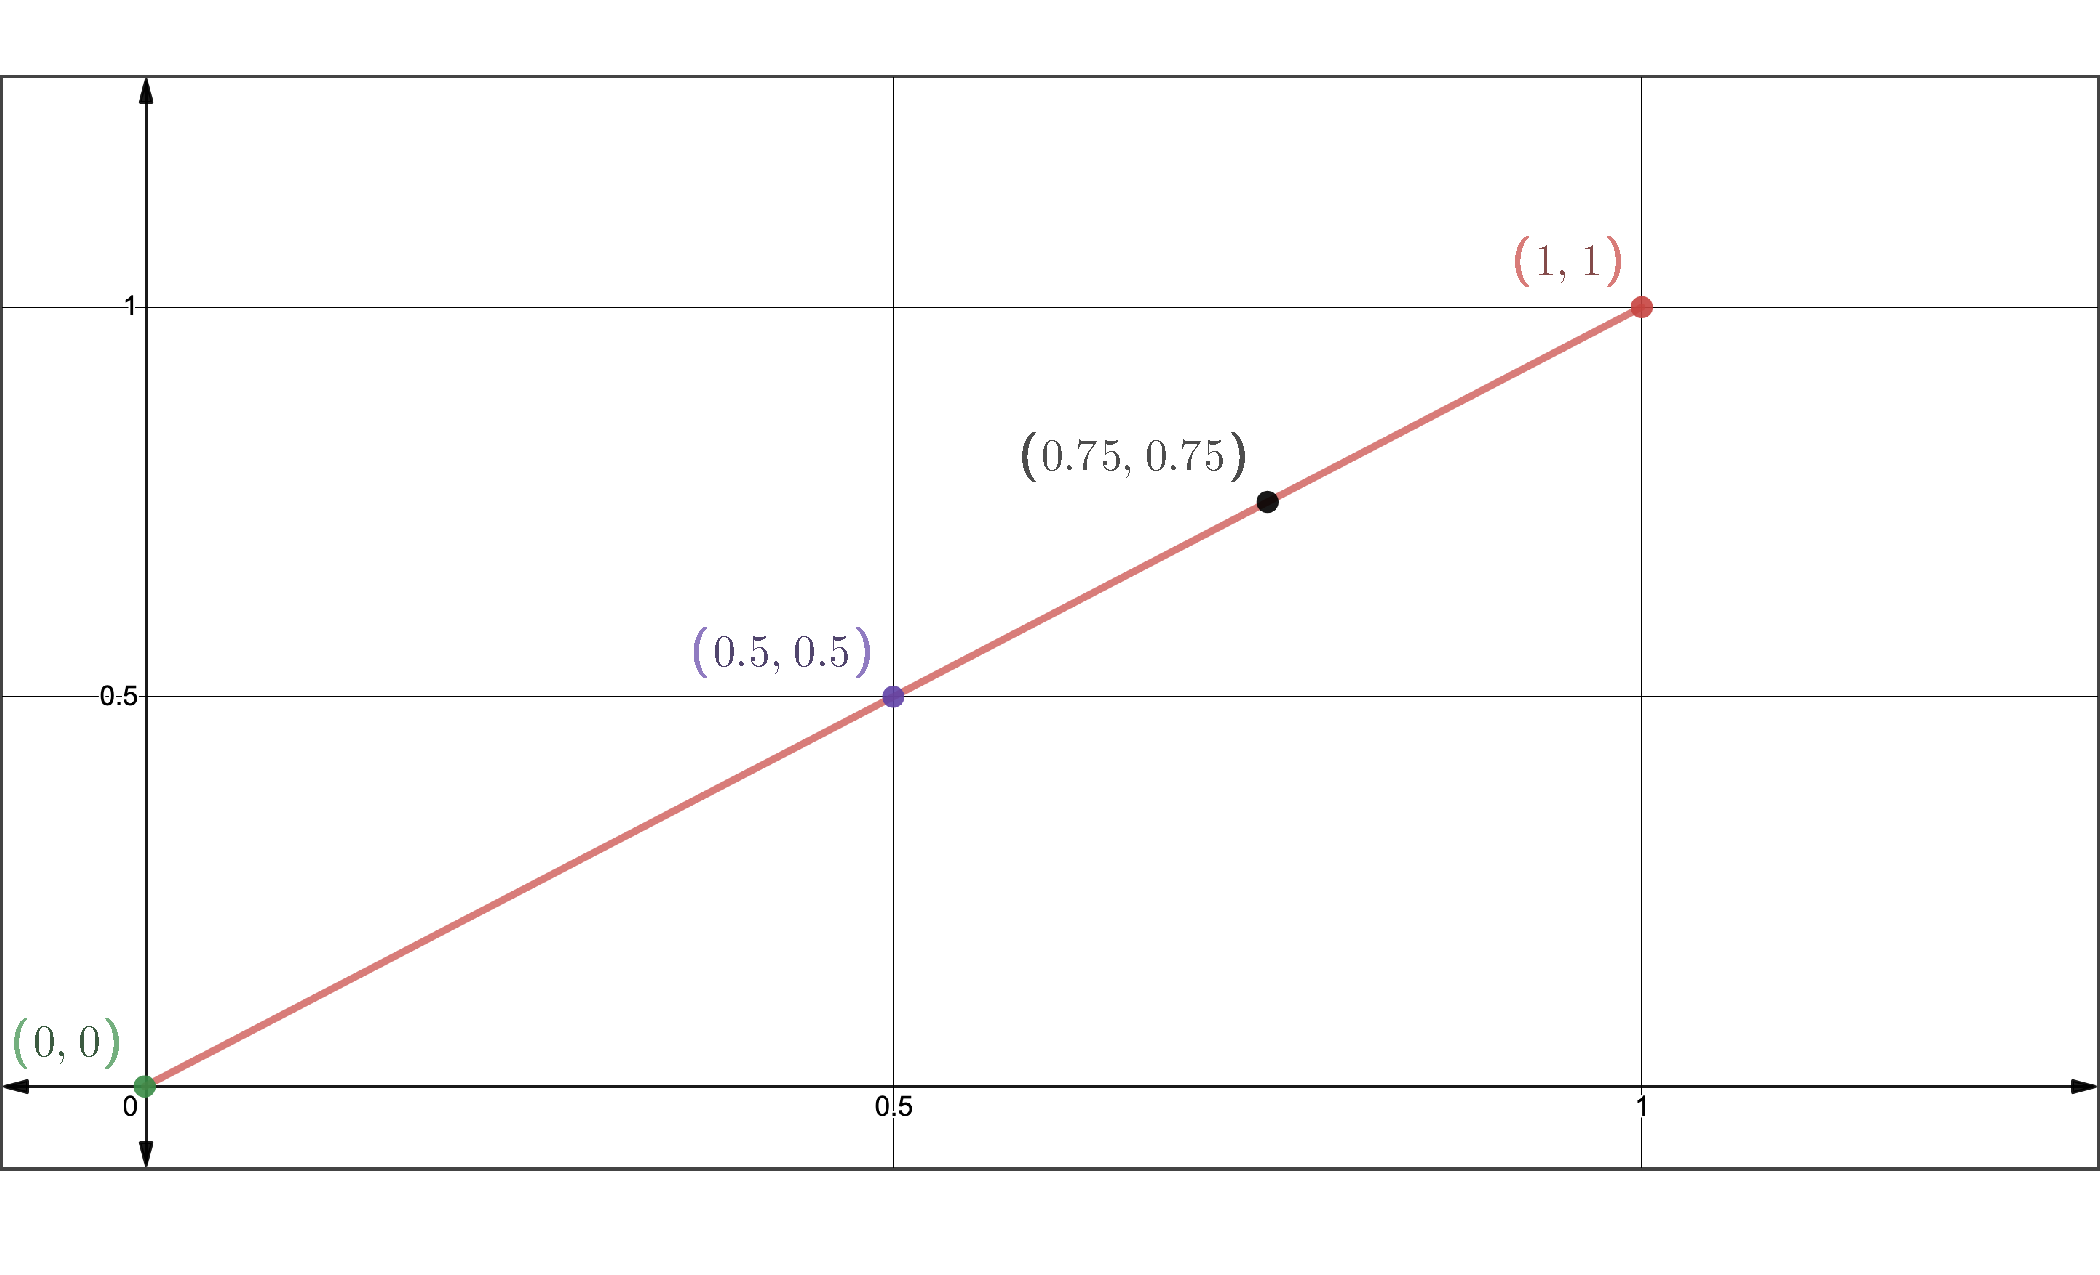
\includegraphics[width=.9\textwidth]{Figures_Part_6/straight_line_curve.pdf}
        		\caption{The curve $\curvegamma(t)$ with labeled points at different times.}
        	\end{figure}
        	In this picture, we can see that the curve begins at the the origin and ends at the point $(1,1)$.  Specifically, we have
        	\[
        	\curvegamma(0) = \begin{pmatrix} 0 \\ 0 \end{pmatrix} \qquad \textrm{and} \qquad \curvegamma(1) = \begin{pmatrix} 1 \\ 1 \end{pmatrix}.
        	\]
        	This curve does not extend indefinitely as our input values can only take on the values in $[0,1]$.
        \end{ex}
        
        From the example, we can see that curves also have a direction associated to them.  As we increase the parameter $t$, we move along the curve in a certain way.  This is an important concept! We can use curves to describe the motion of an object (or other quantities) over time.  This also brings to mind the notion of velocity or speed for a curve.  
        
        \subsection{Derivatives of Curves}
        
        The nice thing about curves is that each component function is a function $\gamma_i\colon \R \to \R$. This means that we can compute the derivatives of each component with the knowledge we have from single variable calculus. In fact, the derivative of a curve can be computed using the typical difference quotient that we learn in a first semester calculus course.  
        
        Imagine that a curve $\curvegamma(t)$ describes the position of a particle at the time $t$.  Then, one could ask for the velocity of this curve which is the first time derivative of position.  Here, we can compute this first derivative at the time $t$ by
        \[
        \tangentgamma(t) = \lim_{\Delta t \to 0} \frac{\curvegamma(t+\Delta t)-\curvegamma(t)}{\Delta t}.
        \]
        We use the overdot notation for $\tangentgamma$ to represent a time derivative of the curve.  We then refer to $\tangentgamma(t)$ as the \boldgreen{tangent vector} to the curve $\curvegamma$ at a time $t$. Now, let us compute the tangent vector explicitly.  We take
        \begin{align*}
        	\tangentgamma(t) &= \lim_{\Delta t \to 0} \frac{\curvegamma(t+\Delta t)-\curvegamma(t)}{\Delta t}\\
        	&= \lim_{\Delta t \to 0} \frac{1}{\Delta t} \left( \begin{pmatrix} \gamma_1(t+\Delta t) \\ \gamma_2(t+\Delta t) \\ \gamma_3(t+\Delta t) \end{pmatrix} - \begin{pmatrix} \gamma_1(t) \\ \gamma_2(t) \\ \gamma_3(t) \end{pmatrix}\right)\\
        	&= \lim_{\Delta t \to 0} \begin{pmatrix} \frac{ \gamma_1(t+\Delta t)-\gamma_1(t)}{\Delta t} \\ \frac{ \gamma_2(t+\Delta t)-\gamma_2(t)}{\Delta t} \\ \frac{ \gamma_3(t+\Delta t)-\gamma_3(t)}{\Delta t} \end{pmatrix}\\
        	&= \begin{pmatrix} \dot{\gamma_1}(t) \\  \dot{\gamma_2}(t) \\ \dot{\gamma_2}(t) \end{pmatrix}.
        \end{align*}
        What this shows is that the tangent vector to a curve $\curvegamma$ is the vector containing the derivative of the components of $\curvegamma$.  Intuitively, this says that the velocity of the curve is found by computing the rate of change of the $x$-component, $y$-component, and $z$-component of $\curvegamma$. 
        
        \begin{ex}{Graph of a Quadratic Function}{graph_quad}
        Consider the curve $\gamma\colon \R \to \R^2$ given by
        \[
        \curvegamma(t)=\begin{pmatrix} t \\ t^2 \end{pmatrix}
        \]
        This curve looks exactly like the graph of the function $f(x)=x^2$ that we have drawn many times before. 
        \begin{figure}[H]
            \centering
            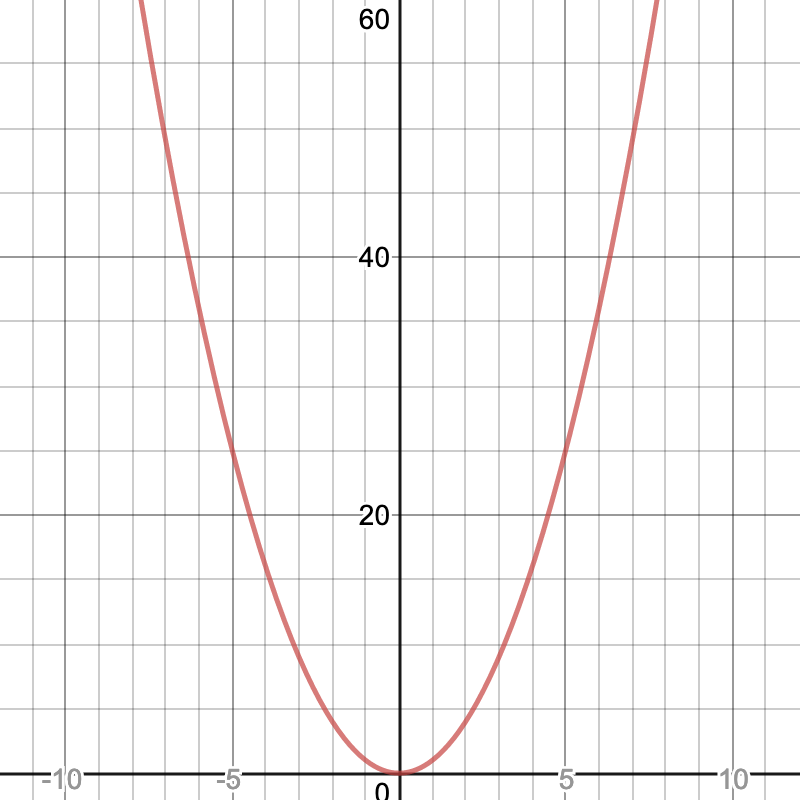
\includegraphics[width=.4\textwidth]{Figures_Part_6/quadratic_curve.png}
        \end{figure}
        What is the tangent vector at time $t$? We have
        \[
        \tangentgamma(t)=\begin{pmatrix} 1 \\ 2t \end{pmatrix}.
        \]
        If we take this $y$-value over the $x$-value we arrive at the same conclusion for the derivative to $f(x)=x^2$ (i.e., $f'(x)=2x$).
        \end{ex}
        
        The two examples of curves we have seen so far mimic graphs of real valued functions we have seen before.  But, curves can be much more general.  There is no need for a curve to pass the horizontal line test, and curves can even have self intersection! For example, a particle that orbits a large body such as the Earth orbits the Sun will move in an elliptical path.  
        
        \begin{ex}{Circle Curve}{circ_curve}
        Consider the curve $\gamma \colon [0,1] \to \R^2$ given by
        \[
        \curvegamma(t)=\begin{pmatrix} \cos (2\pi t) \\ \sin (2\pi t) \end{pmatrix}.
        \]
        This curve is a circle of radius $1$ centered at $(0,0)$.  We can find the tangent vector at a time $t$ by
        \[
        \curvegamma(t)=\begin{pmatrix} -2\pi \sin(2\pi t) \\ 2\pi \cos(2\pi t)\end{pmatrix}.
        \]
        See the following graphs
        
    \begin{figure}[H]
    \centering
    \begin{subfigure}[h]{0.45\textwidth}
        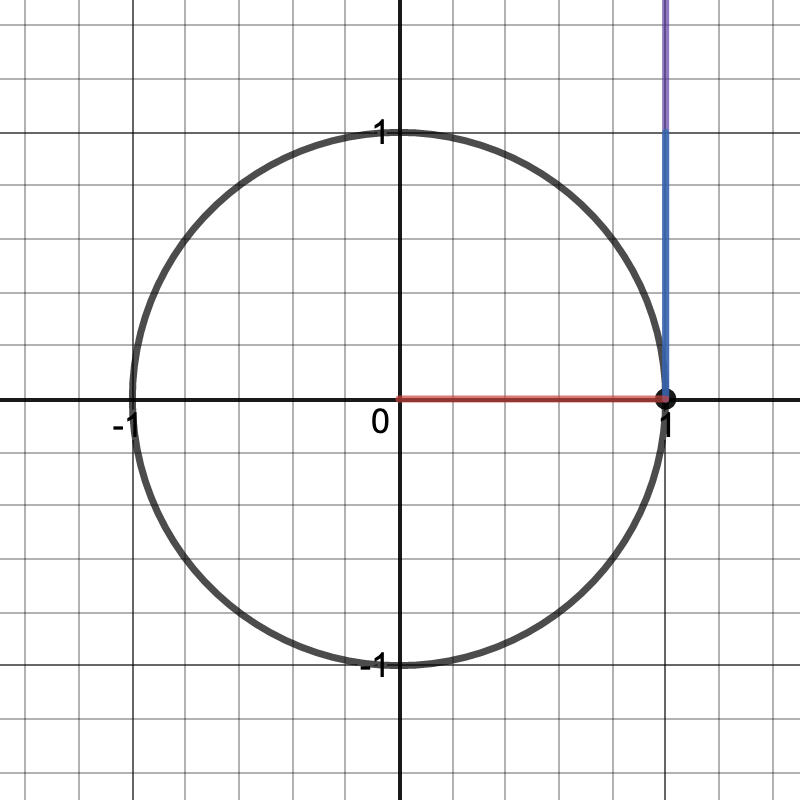
\includegraphics[width=\textwidth]{Figures_Part_6/circ_tang_1.png}
        \caption{Tangent vector at $t=0$.}
    \end{subfigure}
    ~ 
    \begin{subfigure}[h]{0.45\textwidth}
        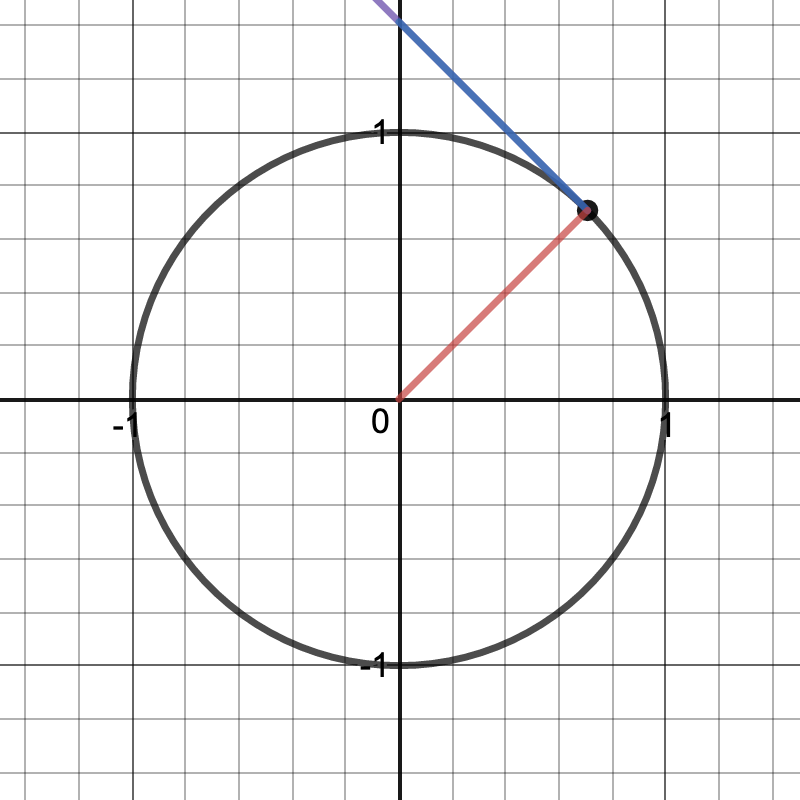
\includegraphics[width=\textwidth]{Figures_Part_6/circ_tang_2.png}
        \caption{Tangent vector at $t=\frac{1}{8}$.}
    \end{subfigure}
    
    \begin{subfigure}[h]{0.45\textwidth}
        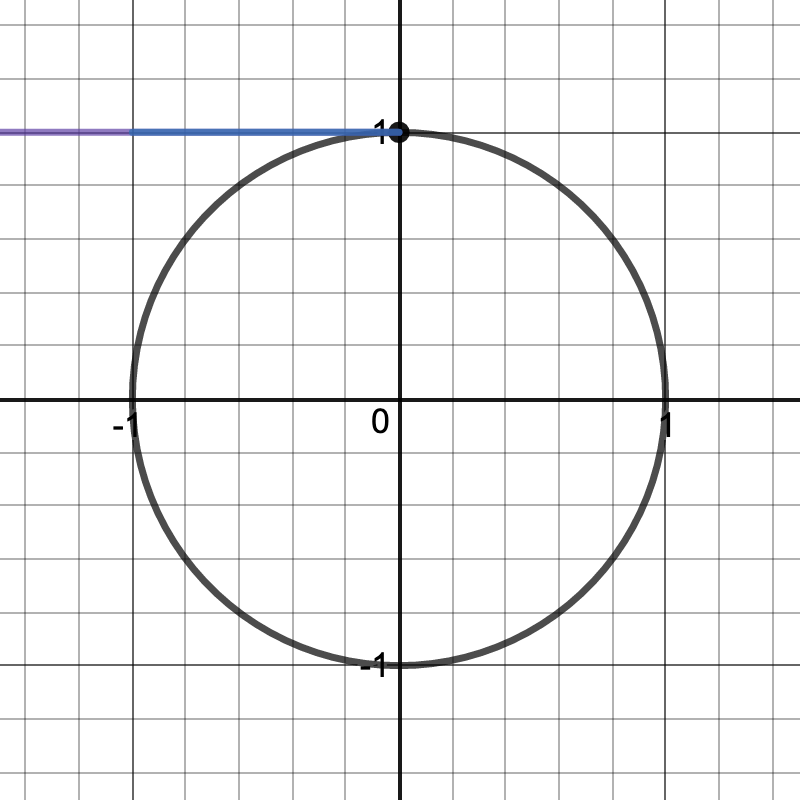
\includegraphics[width=\textwidth]{Figures_Part_6/circ_tang_3.png}
        \caption{Tangent vector at $t=\frac{1}{4}$.}
    \end{subfigure}
    ~
    \begin{subfigure}[h]{0.45\textwidth}
        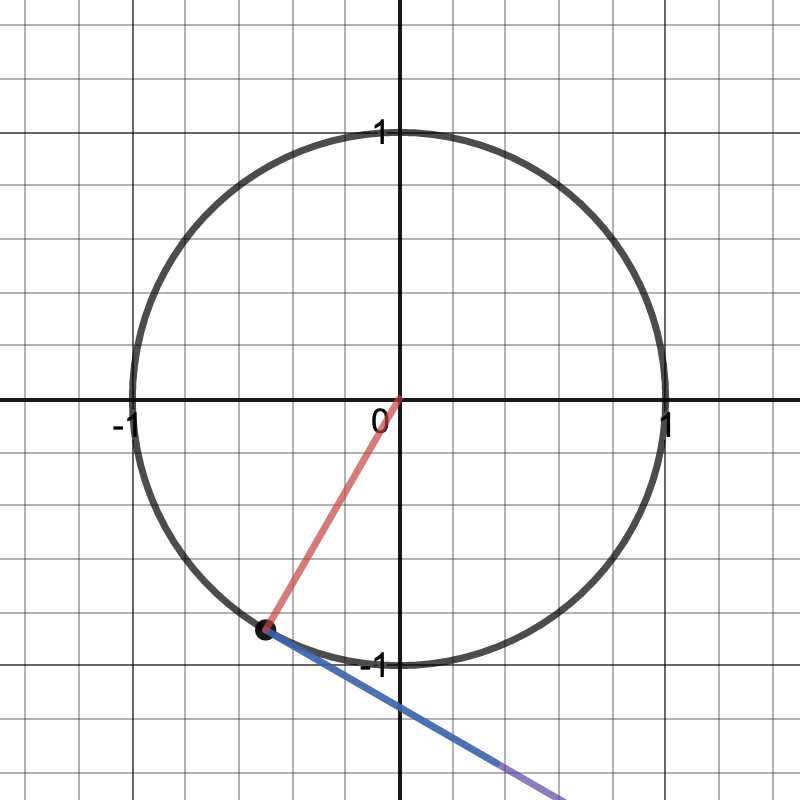
\includegraphics[width=\textwidth]{Figures_Part_6/circ_tang_4.png}
        \caption{Tangent vector at $t=\frac{2}{3}$.}
    \end{subfigure}
        \end{figure}
        \end{ex}
        
        There is nothing stopping us from computing the second time derivative of a curve as well.  We repeat the process for computing the first derivative above, but instead we take the time derivative of the tangent vector $\tangentgamma$.  This yields,
                \[
                \normalgamma(t) = \begin{pmatrix} \ddot{\gamma_1}(t) \\ \ddot{\gamma_2}(t) \\ \ddot{\gamma_3}(t) \end{pmatrix}.
                \]
         We then refer to this quantity as the \boldgreen{normal vector} to the curve $\curvegamma$. 
         
         \begin{exercise}
         	Compute the normal vector to the circle curve in the previous exercise.  If you know of the notion of centripetal force, how does this quantity relate?
         \end{exercise}
         
         \subsection{Lengths of Curves}
        
        Integration is a tool we use to add up values of functions.  In the 1-dimensional case, we found that the integral of a function $f(x)$ from $x=a$ to $x=b$ computed the net area under the graph of the function.  Similarly, we can use integration to compute the length of a curve.
        
        If we take a curve $\curvegamma \colon [a,b] \to \R^3$, then we can compute the tangent vector at time $t$, $\tangentgamma(t)$. Again, the tangent vector is analogous to the velocity of a curve (at some point in time), and so the length of this tangent vector is the speed.  So, we put that the speed of the curve at time $t$ is $\left| \tangentgamma(t)\right|$.  
        
        Computing the length of a curve amounts to adding up the speed of the curve over the total amount of time.  In this perspective, this just takes into account the total distance a particle has moved, even if the particle back-tracks at some point. We can write this length as
        \[
        \ell(\curvegamma) = \int_a^b \left|\tangentgamma(t)\right|dt.
        \]
        
        \begin{ex}{Circumference of a Circle}{circ_of_circ}
        	Take for example the circle curve $\curvegamma \colon [0,1] \to \R^2$ given by
        	\[
        	\curvegamma(t) = \begin{pmatrix} \cos(2\pi t) \\ \sin(2\pi t) \end{pmatrix}.
        	\]
        	Then, we found 
        	\[
        	\tangentgamma(t) = \begin{pmatrix} -2\pi \sin(2\pi t) \\ 2\pi \cos(2 \pi t) \end{pmatrix}.
        	\]
        	Taking the length of the tangent vector at time $t$ yields
        	\[
        	\left| \tangentgamma(t) \right| = \sqrt{4\pi^2 \sin^2(2\pi t) + 4\pi^2 \cos^2(2\pi t) } = 2\pi.
        	\]
        	The length is then
        	\[
        	\ell(\gamma) = \int_0^1 2 \pi t  = 2\pi,
        	\]
        	which is indeed the circumference of a circle of radius one.
        \end{ex}
                
                \section{Scalar fields}
                The next major class of functions we will consider are the scalar fields.  That is, functions that take the form
                \[
                f\colon \R^3 \to \R.
                \]
                Often, it will be helpful to visualize functions by considering instead
                \[
                f\colon \R^2 \to \R
                \]
                and looking at the \boldgreen{graph} of $f$.  
                
                \begin{ex}{Graph of a function}{graph_of_func}
                Whenever we talk of a function of the form
                \[
                f\colon \R \to \R
                \]
                we inherently tend to draw the graph of the function $f$.  By graph, I mean that given $f$, we usually just draw $(x,f(x))$ in the plane.
                
                Take for example, $f\colon \R \to \R$ given by $f(x)=x^2$.  We usually draw the plane $\R^2$ and graph the curve $(x,f(x))$ which looks like
                \begin{figure}[H]
                    \centering
                    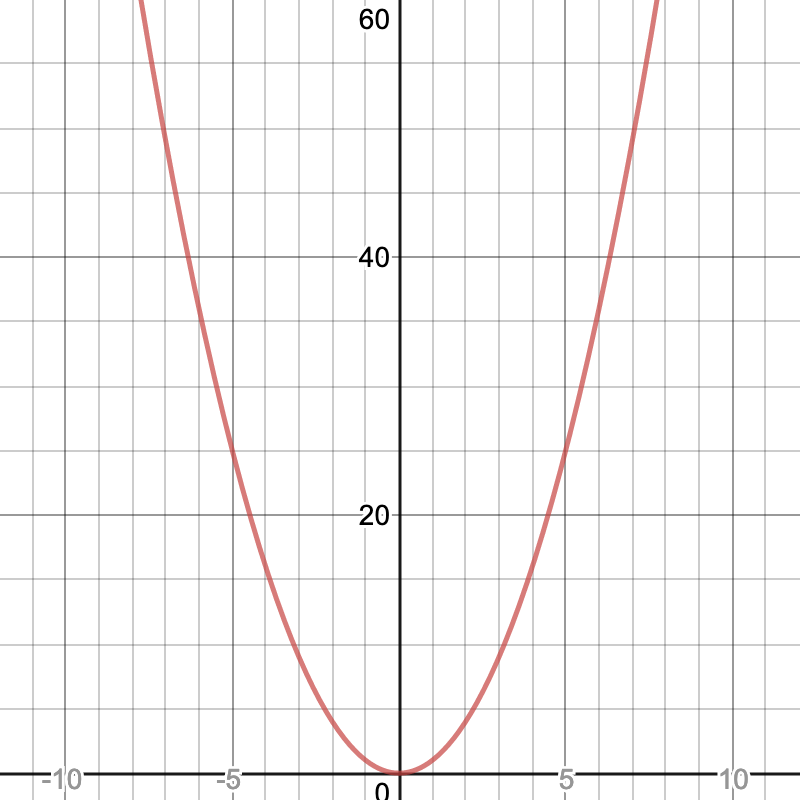
\includegraphics[width=.5\textwidth]{Figures_Part_6/quadratic_curve.png}           
                \end{figure}
                All of this is to say that graphs of these types of functions are special kinds of curves.  In other words, they are curves that pass the vertical line test. 
                \end{ex}
                
                The 1-dimensional examples are rather redundant.  In a vague sense, it's hard to differentiate between 1-dimensional curves, scalar fields, and vector fields.  However, if we consider graphing higher dimensional scalar fields, we will immediately see a difference.  Our new point of view will be to look at the graph of 2-dimensional scalar fields in order to gain intuition on the 3-dimensional scalar fields.  
                
                Graphing a 1-dimensional scalar field $f$ involved plotting the graph
                \[
                (x,f(x)).
                \]
                Here, we put the $y$-component of the output as the function $f(x)$ which allows us to see the function values at a point $x$ as the height above (or below) the $x$-axis. Similarly, if we have a scalar field $h(x,y)$, we can plot the set of points
                \[
                (x,y,h(x,y)),
                \]
                in 3-dimensional space.  Then, what we receive is a picture that places $z=h(x,y)$ so that we see the function $h$ describing the height of a sheet above the $xy$-plane.
                
                \begin{ex}{The Paraboloid}{paraboloid}
                Let $f\colon \R^2 \to \R$ be given by
                \[
                f(x,y)=x^2+y^2.
                \]
                We can plot the graph of the function by plotting $(x,y, f(x,y))$ in $\R^3$.  This will look like:
                \begin{figure}[H]
                    \centering
                    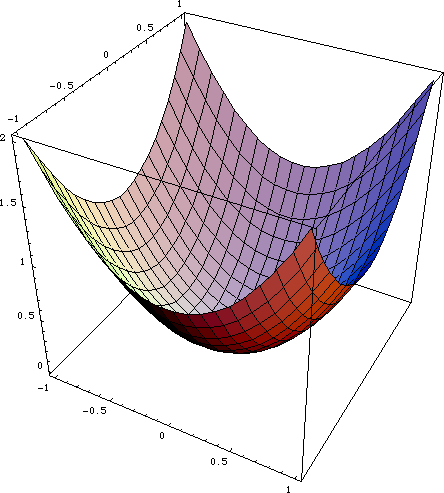
\includegraphics[width=.4\textwidth]{Figures_Part_6/paraboloid.png}
                \end{figure}
                Then we can analyze this function in a few nice ways.  
                
                If we fix a value for $x$ or $y$, then we will be able to look at $f$ as a function of just a single variable.  
                \begin{itemize}
                \item So we can, for example, fix $y=0$ and then we have
                \[
                f(x,0)=x^2.
                \]
                So along the $y=0$ line, the function is just the parabola we are used to! 
                
                \item Similarly, we can force $x=0$ and arrive at
                \[
                f(0,y)=y^2
                \]
                is also a parabola.  
                
                \item But we are not limited to these choices.  We could have chosen $y=5$ and we would have
                \[
                f(x,5)=x^2+25
                \]
                which is a parabola shifted upwards by 25 units.
                
                \item  Again, we could also choose yet another ``slice" of this function and let $x=y$ which would give us
                \[
                f(x,x)=x^2+x^2=2x^2.
                \]
                So, along the $x=y$ line, the parabola is scaled by 2.
                
	                \item One other method of analyzing this function would be to find what the \boldgreen{level curves} of this function are.  What are the points $(x,y)$ that satisfy $f(x,y)=c$?  We call these level curves much in the way that a topographical map plots curves along the areas with equal height.  For this example, consider the set of points $(x,y)$ so that $f(x,y)=1.$ This means
                \[
                f(x,y)=1=x^2+y^2.
                \]
                Since we have
                \[
                x^2+y^2=1
                \]
                that means each level curve is a circle!
                \item Here is a ``topographical map" for this function (i.e., a plot of the level curves for this paraboloid.)
                \begin{figure}[H]
                    \centering
                    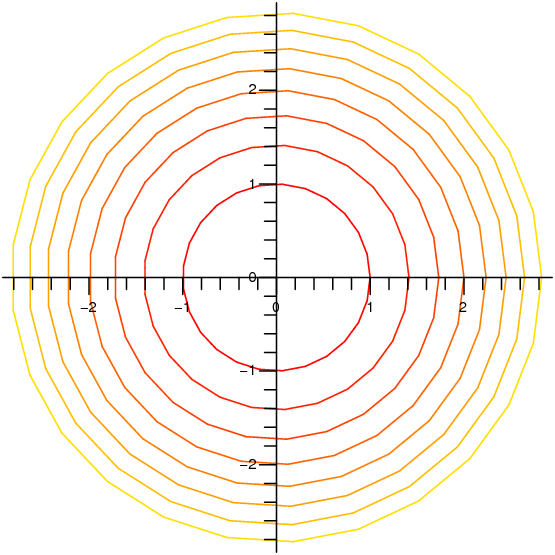
\includegraphics[width=.4\textwidth]{Figures_Part_6/parabolic_level_curves.png}
                \end{figure}
                Here, each circle represents $f(x,y)=c$ for different values of $c$.  This really \emph{is} a topographical map!
                \end{itemize}
                \end{ex}
                
                \begin{exercise}[Plane]
                Repeat this analysis for yourself for the following function:
                \[
                f(x,y)=x+y.
                \]
                \end{exercise}
                
                An important remark is that we should only use this idea to gain intuition. For one, it fails when our function is given by $f\colon \R^n \to \R$ where $n>2$.  The objects for calculus that we develop for scalar fields do not take into account the graph of the function, but just the function itself.  
                
                \subsubsection{Derivatives of scalar fields}
                        We can investigate functions of multiple variables in more ways than the single variable case.  Let us start with scalar fields.
                        
                        \begin{df}{Partial Derivatives}{partial_derivs}
                        Let $f\colon \R^3 \to \R$ be a scalar field.  Then we can consider derivatives with respect to changing each input.  For example, we define the \boldgreen{partial derivative with respect to $x$} \boldgreen{at the point $(x_0,y_0,z_0)$}, denoted $\frac{\partial f}{\partial x}(x_0,y_0,z_0)$, and put
                        \[
                        \frac{\partial f}{\partial x}(x_0,y_0,z_0)\coloneqq \lim_{\delta \to 0} \frac{f(x_0+\delta,y_0,z_0)-f(x_0,y_0,z_0)}{\delta}
                        \]
                        \end{df}
                       
                        
                        \begin{remark}
                        For partial derivatives, all but one variable are being held constant.  So, when you are computing these, be sure to treat the proper variables as constant when necessary.
                        \end{remark}
                        
                        To make notation easier to deal with, we will often just write 
                        \[
                        \frac{\partial f}{\partial x}
                        \]
                        in place of
                        \[
                        \frac{\partial f}{\partial x}(x,y,z).
                        \]
                        When we specify a point at which this partial derivative should be computed, then we must use the notation
                        \[
                         \frac{\partial f}{\partial x}(x_0,y_0,z_0),
                        \]
                        so that the meaning is unambiguous.
                        
                        \begin{exercise}
                        Define $\frac{\partial f}{\partial y}$ and $\frac{\partial f}{\partial z}$ in a similar way to the above definition.
                        \end{exercise}
                        
                        \begin{exercise}
                        Compute $\partialx$, $\partialy$, and $\partialz$ for the function 
                        \[
                        f(x,y,z)=\sin(xyz)+x+2y^2+3x^2z.
                        \]
                        \end{exercise}
                        
                        It turns out that collecting the partial derivatives as a vector is the best linear approximation to a scalar function.  We call this vector the gradient vector.
                        
                        \begin{df}{The Gradient}{gradient}
                        Given a scalar field $f(x,y,z)$, the \boldgreen{gradient of $f$ at the point $(x_0,y_0,z_0)$}, denoted $\grad f(x_0,y_0,z_0)$ is given by
                        \[
                        \grad f(x_0,y_0,z_0)=\begin{pmatrix} \partialx(x_0,y_0,z_0)\\ \partialy(x_0,y_0,z_0)\\ \partialz(x_0,y_0,z_0)\end{pmatrix}.
                        \]
                        \end{df}
                        
                        In fact, we often will consider the gradient as a vector itself.  That is, we will put
                        \[
                        \grad = \begin{pmatrix} \partialwrt{x} \\ \partialwrt{y} \\ \partialwrt{z} \end{pmatrix}.
                        \]
                        This will allow us to compute derivatives of vector fields by use of the cross and dot products.
                        
                        \begin{exercise}
                        Compute the gradient for the function
                        \[
                        f(x,y,z)=\sin(xyz)+x+2y^2+3x^2z.
                        \]
                        \end{exercise}
                        
                        \subsubsection{Properties of partial derivatives and the gradient}
                        
                        As with the one-dimensional derivative, we have some properties that will be helpful.\\
                        
                        \noindent\textbf{Partial Derivatives:}
                        \begin{enumerate}[(i)]
                            \item \textbf{Sum Rule:} Given $f(x,y,z)$ and $g(x,y,z)$, we have that
                            \[
                            \frac{\partial}{\partial x} (f(x,y,z)+g(x,y,z))=\partialx + \frac{\partial g}{\partial x}.
                            \]
                            Of course, this holds for any partial derivative.
                            \item \textbf{Constant Multiple:} Given $\lambda \in \R$ and $f(x,y,z)$, we have that
                            \[
                            \frac{\partial}{\partial x}(\lambda f(x,y,z))=\lambda \partialx.
                            \]
                            Again, this holds for any partial derivative.
                            \item \textbf{Product Rule:} Given $f(x,y,z)$ and $g(x,y,z)$ we have that
                            \[
                            \frac{\partial }{\partial x}(f(x,y,z)g(x,y,z))=\partialx g + f \frac{\partial g}{\partial x}.
                            \]
                            Ths holds for all partial derivatives.
                        \end{enumerate}
                        
                        \begin{remark}
                        The chain rule will show up eventually, but not yet.  As for the quotient rule, this also holds, but I don't show it here.
                        \end{remark}
                        
                        \noindent\textbf{The Gradient:}
                        \begin{enumerate}[(i)]
                            \item \textbf{Sum Rule:} Given $f(x,y,z)$ and $g(x,y,z)$, we have that
                            \[
                            \grad(f(x,y,z)+g(x,y,z))=\grad f(x,y,z)+\grad g(x,y,z).
                            \]
                            \item \textbf{Constant Multiple:} Given $\lambda \in \R$ and $f(x,y,z)$, we have that
                            \[
                            \grad(\lambda f(x,y,z))=\lambda \grad f(x,y,z).
                            \]
                            \item \textbf{Product Rule:} Given $f(x,y,z)$ and $g(x,y,z)$ we have that
                            \[
                            \grad(f(x,y,z)g(x,y,z))=(\grad f(x,y,z))g(x,y,z)+f(x,y,z)(\grad g(x,y,z))
                            \]
                            
                        \end{enumerate}
                        
                        We've learned how to compute partial derivatives and the gradient, but what are they really telling us? Remember that the derivative $\frac{d}{dx}$ of a function $f(x)$ tells us the rate of change of $f$ as we move in the $x$-direction.  This is very similar to what $\frac{\partial}{\partial x}$ tells us about a function $f(x,y,z)$.  So we can say the following.
                        \begin{itemize}
                            \item $\frac{\partial f}{\partial x}$ tells us how $f$ changes as we move in the $x$-direction.
                            \item $\frac{\partial f}{\partial y}$ tells us how $f$ changes as we move in the $y$-direction.
                            \item $\frac{\partial f}{\partial z}$ tells us how $f$ changes as we move in the $z$-direction.
                        \end{itemize}
                        
                        We can put these together into the gradient $\nabla f$ and know how $f$ changes in each possible direction. Let's see how the gradient acts then. 
                        
                        \begin{ex}{Gradients on the Paraboloid}{gradients_paraboloid}
                        Let us start with $f(x,y)=x^2+y^2$.  Then
                        \[
                        \nabla f(x,y) = (2x,2y).
                        \]
                        Let us plot the level curves of this surface.
                        \begin{figure}[H]
                            \centering
                            \begin{subfigure}[h]{.45\textwidth}
                            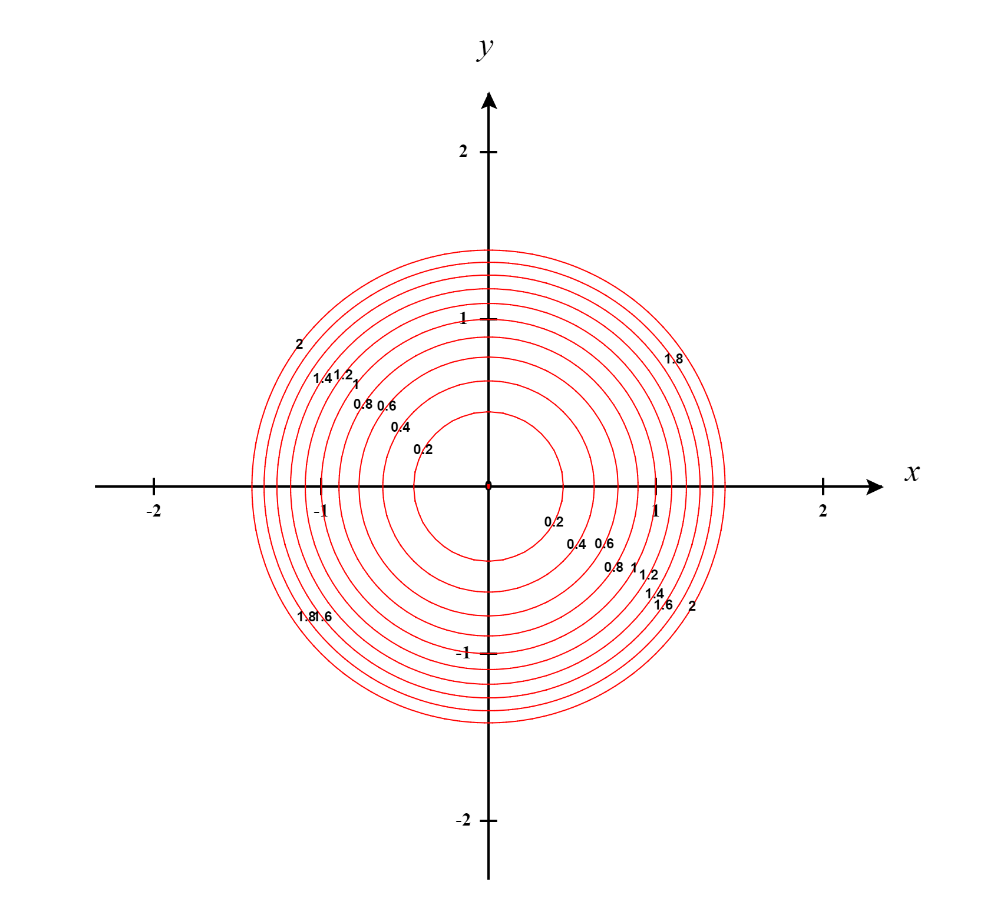
\includegraphics[width=\textwidth]{Figures_Part_6/level_curves_gradient.png}
                            \caption{Level curves of $f(x,y)$.}
                            \end{subfigure}
                            ~
                            \begin{subfigure}[h]{.45\textwidth}
                            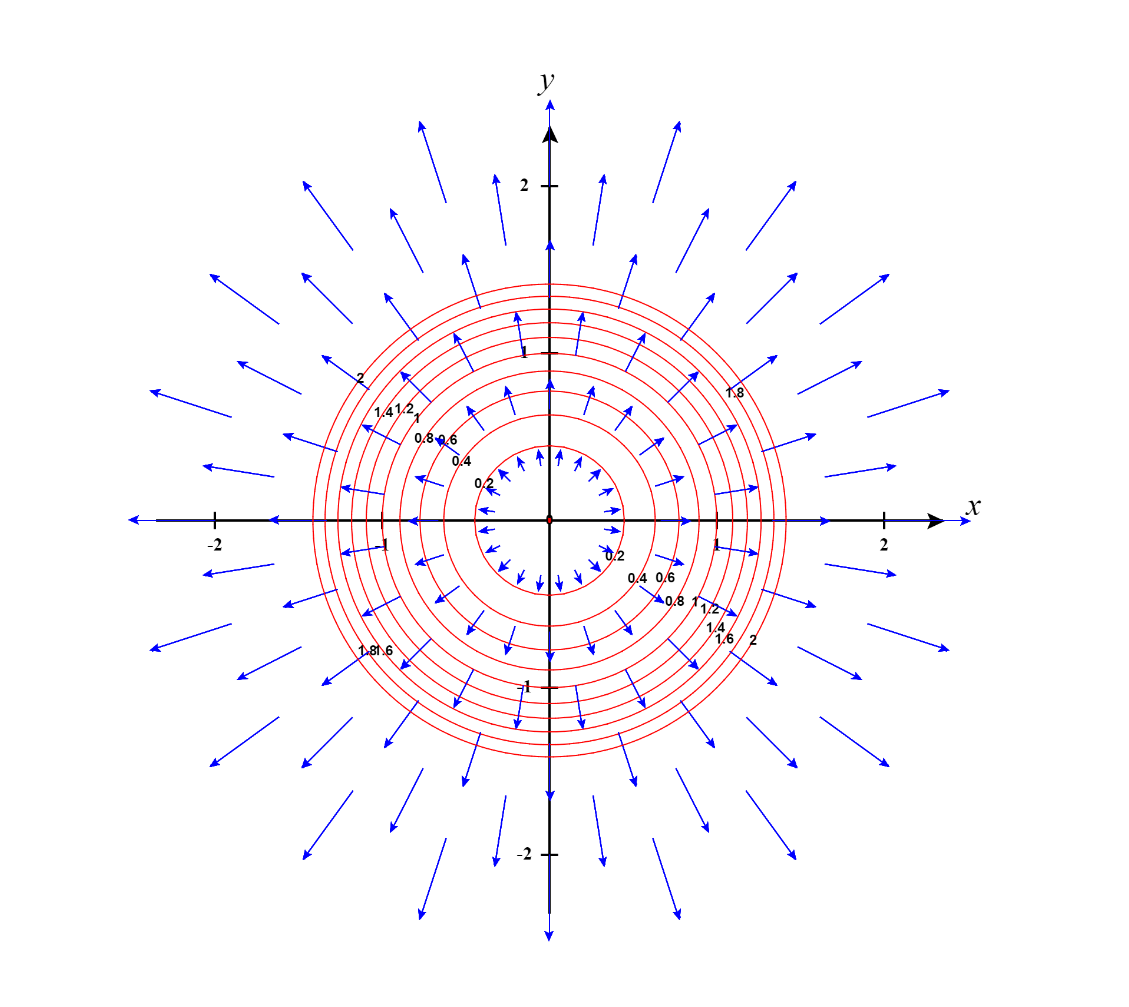
\includegraphics[width=\textwidth]{Figures_Part_6/level_curves_gradient_vectors.png}
                            \caption{Gradient vectors shown in blue.}
                            \end{subfigure}
                        \end{figure}
                        \begin{itemize}
                            \item Notice that the gradient vectors point in a direction perpendicular to the level curves and the length corresponds to how close the nearest level curve is.
                            \item The gradient is zero at the bottom of this surface.  
                        \end{itemize}
                        \end{ex}
                        
                        \begin{prop}{Gradient Points Uphill}{gradient_prop}
                        The gradient $\nabla f(x,y,z)$ is the vector that points in the direction of greatest increase for a function $f(x,y,z)$.
                        \end{prop}
                        
                        How about second partial derivatives? What can we say here. We have each of the following for a function $f(x,y)$:
                        \begin{itemize}
                            \item $\frac{\partial^2 f}{\partial x^2}$
                            \item $\frac{\partial^2 f}{\partial y^2}$
                            \item $\frac{\partial}{\partial y}\frac{\partial f}{\partial x}$
                            \item $\frac{\partial}{\partial x}\frac{\partial f}{\partial y}$
                        \end{itemize}
                        
                        Recall what $\frac{d^2 f}{dx^2}$ meant for a function $f(x)$.  This told us how $f$ was curving (or what concavity $f$ had). The story is similar for these partial derivatives.
                        
                        \begin{itemize}
                            \item $\frac{\partial^2 f}{\partial x^2}$ tells us about the concavity (or curvature) of $f$ as we move in the $x$ direction.
                            \item $\frac{\partial^2 f}{\partial y^2}$ tells us about the concavity (or curvature) of $f$ as we move in the $y$ direction.
                            \item We actually have that $\frac{\partial}{\partial y}\frac{\partial f}{\partial x}=\frac{\partial}{\partial x}\frac{\partial f}{\partial y}$.  This interpretation is a bit hard to deal with.  Let's not worry too much about it.
                        \end{itemize}
                        
                        \begin{prop}{Partial Derivatives Commute}{partials_commute}
                        We have that
                        \[
                        \frac{\partial}{\partial y}\frac{\partial f}{\partial x}=\frac{\partial}{\partial x}\frac{\partial f}{\partial y}.
                        \]
                        Moreover, for functions of more variables, we can say that the order we take derivatives does not matter.
                        \end{prop}
                        
                        \begin{exercise}
                        Given $f(x,y)=x^2+y^2$, compute
                        \[
                        \frac{\partial^2 f}{\partial x^2}, ~ \frac{\partial^2 f}{\partial y^2}, ~ \frac{\partial}{\partial y}\frac{\partial f}{\partial x},~ \frac{\partial}{\partial x}\frac{\partial f}{\partial y}.
                        \]
                        What can we say about the curvature of $f$ in the two directions? Does this make sense?
                        \end{exercise}
                        
                        \subsection{Directional Derivatives}
                        
                        Related to the notion of partial differentiation and the gradient is that of finding the derivative of a function in a given direction.  Say that we are given a scalar field $f(x,y,z)$, and we are also given a unit vector $\unitvec$.  Then, we can compute the \boldgreen{directional derivative of $f$ in the direction $\unitvec$} by
                        \[
                        \frac{\partial f}{\partial \unitvec} = \unitvec \cdot \grad f.
                        \]
                        There is another way to define this derivative, but it requires a bit more work to derive.
                        
                                               
                        One can see that we can recover partial derivatives via this notion as well.  For example, if we let $\unitvec = \xhat$, then we have
                        \[
                        \frac{\partial f}{\partial \unitvec} = \xhat \cdot \grad f = \partialx.
                        \]
                        We can think of directional derivatives as generalizations of partial derivatives where we allow for computing the derivative of our function $f$ in a direction other than the ones given by the chosen basis.
                        
                        \section{Optimization}
                        In single variable calculus, we optimized functions $f(x)$ by finding the point $x_0$ where 
                        \[
                        f'(x_0)=0.
                        \]
                        We called this a \emph{critical point}. We found if this optimizer $x_0$ was a maximizer or minimizer by checking the sign of second derivative $f''(x_0)$. We had
                        \begin{align*}
                            \textrm{Maximum: }& f''(x_0)<0\\
                            \textrm{Minimum: }& f''(x_0)>0.
                        \end{align*}
                        
                        In higher dimensions, this idea works similarly. We just have more to check. 
                        
                        \begin{df}{Stationary Points}{stationary_points}
                        Given a function $f(x,y)$, we call a point $(x_0,y_0)$ a \textbf{stationary point} if 
                        \[
                        \nabla f(x_0,y_0) = \mathbf{0}.
                        \]
                        \end{df}
                        
                        As before, we will use second derivatives to find out whether this is a maximum or a minimum.
                        
                        \begin{prop}{Maximizers and Minimizers}{max_min}
                        A stationary point $(x_0,y_0)$ is a 
                        \begin{align*}
                            \textrm{Maximizer if~ }& \frac{\partial^2 f}{\partial x^2} <0 \textrm{ ~and~ } \frac{\partial^2 f}{\partial y^2}<0,\\
                            \textrm{Minimizer if~ }& \frac{\partial^2 f}{\partial x^2} >0 \textrm{ ~and~ } \frac{\partial^2 f}{\partial y^2}>0,\\
                            \textrm{Saddle if otherwise.}
                        \end{align*}
                        \end{prop}
                        
                        \begin{exercise}
                        Let
                        \[
                        f(x,y) = \frac{xy}{e^{x^2+y^2}}.
                        \]
                        \begin{enumerate}[(a)]
                            \item Find all stationary points for $f$.
                            \item Determine whether these points are minimizers or maximizers.
                        \end{enumerate}
                        \end{exercise}
                        
                        \begin{exercise}
                        Show that $f(x,y)=xy$ has a saddle point at $(0,0)$.
                        \end{exercise}
                        
                        Some optimization problems cannot be solved just using this technique.  If you are interested, consider reading about \boldgreen{Lagrange multipliers}.
                        
%                        \subsubsection{Lagrange Multipliers}
%                        Often times we are given a situation that we wish to find an optimum solution to, but we are somehow constrained.  A biological example would be fixing a given volume for a red blood cell, and finding the optimum shape so that oxygen diffusion is maximized.  A physical example would be finding the fastest path between two points when moving through a medium with varying viscosity.
%                        
%                        The idea is relatively tame. We are given the function to optimize
%                        \[
%                        f(x,y,z)
%                        \]
%                        and the constraining function
%                        \[
%                        g(x,y,z)=k.
%                        \]
%                        Then we must solve the equation
%                        \[
%                        \nabla f(x,y,z) = \lambda \nabla g (x,y,z)
%                        \]
%                        where $\lambda$ is called the \textbf{Lagrange multiplier}. Let's work through an example of solving this.
%                        
%                        \begin{ex}{Largest Box}{largest_box}
%                        Let's find the dimensions of the box with the largest volume if the total surface area is $64 cm^2$.  We must determine our function to optimize, which is the volume function
%                        \[
%                        V(x,y,z) = xyz.
%                        \]
%                        Our constraint is the surface area function $A(x,y,z)$ must be
%                        \[
%                        g(x,y,z)=2xy+2xz+2yz=64,
%                        \]
%                        which we will simplify as
%                        \[
%                        xy+xz+yz = 32.
%                        \]
%                        \begin{enumerate}
%                            \item We first take
%                            \[
%                            \nabla f(x,y,z) = \begin{bmatrix} yz \\ xz \\ xy \end{bmatrix}
%                            \]
%                            and
%                            \[
%                            \nabla g(x,y,z) = \begin{bmatrix} 2y+2z \\ 2x+2z \\ 2x+2y\end{bmatrix}.
%                            \]
%                            \item This gives us four equations to solve. Three are from the equation $\nabla f(x,y,z) =\nabla g(x,y,z)$
%                            \begin{align}
%                                yz &= \lambda (y+z)\\
%                                xz &= \lambda (x+z)\\
%                                xy &= \lambda (x+y),
%                            \end{align}
%                            and one is from the constraint $g(x,y,z)=64$
%                            \[
%                            xy+xz+yz = 32.
%                            \]
%                            \item Working through solving these can be nontrivial.  In this case, we can do the following: Multiply (1) by $x$, (2) by $y$, and $(3)$ by $z$.  Which gives us
%                            \begin{align*}
%                                xyz &= \lambda x(y+z)\\
%                                xyz &= \lambda y(x+z)\\
%                                xyz &= \lambda z(x+y)
%                            \end{align*}
%                            Now we can set the first two equal to find
%                            \[
%                            \lambda x(y+z)=\lambda y(x+z)
%                            \]
%                            which simplifies to 
%                            \[
%                            \lambda (xz-yz)=0
%                            \]
%                            meaning that $\lambda =0$ or $xz=yz$. Note that $\lambda =0$ is not possible since that will end up giving us zero surface area and we won't satisfy the constraint.
%                            
%                            Now $xz-yz=0$ means that $x=y$, which we can substitute back into the equations later. 
%                            
%                            We can set the last two equal to find
%                            \[
%                            \lambda y (x+z)=\lambda z(x+y)
%                            \]
%                            which with similar work tells us $z=y$.  So now we make note of $x=y$ and we have $x=y=z$.  
%                            
%                            So now we use the constraint equation with $x=y=z$ and find that we have
%                            \[
%                            x^2+y^2+z^2 = 3x^2 = 32
%                            \]
%                            which means that $x\approx 3.266$.  Thus
%                            \[
%                            V(3.266,3.266,3.266)\approx 34.8376
%                            \]
%                            is the largest volume.  \emph{This means our ideal solution is a cube!} 
%                            
%                        \end{enumerate}
%                        \end{ex}
                        
                       
                
                
                \section{Integrals of Scalar Fields}
                
                In one dimension, we integrated functions in order to sum up values over a given interval.  Geometrically, this gave us the net area under a curve.  In this case, we took a function $f(x)$ and an interval $[a,b]$ and we wrote
                \[
                \int_a^b f(x) dx.
                \]
                When we work in higher dimensions, we have to be a bit more careful.  Let us instead rephrase this problem by instead specifying a region $\Omega = [a,b]$ and a function $f$, then we would put
                \[
                \int_\Omega f d\Omega = \int_a^b f(x)dx.
                \]
                The difference we wish to establish is that the integral we are performing depends on the coordinates in which we choose.  Later on, this will become very apparent when we consider new forms of coordinate systems (e.g., polar coordinates).  
                
                What we put above is simply a change of notation that allows for greater versatility.  Imagine we have a region in the plane $\Omega$ and a scalar field $f\colon \Omega \to \R$, then we can plot the graph of that function in Cartesian coordinates by thinking of the function $f$ as taking in an $(x,y)$ pair, and placing $f(x,y)$ as the height above the $xy$-plane.
                \begin{figure}[H]
                	\centering
                	\def\svgwidth{0.75\columnwidth}
                	\input{Figures_Part_6/surface_graph.pdf_tex}
                \end{figure}
                A region $\Omega$ is given in the plane with respect to some coordinates.  For example, we may specify the region in the plane by $x_0 \leq x \leq x_1$ and $y_0 \leq y \leq y_1$, and so we write our function with respect to these choices.  Then, say we want to compute the volume under the surface given by the graph $(x,y,f(x,y))$, we would then compute
                \[
                \int_{y_0}^{y_1} \int_{x_0}^{x_1} f(x,y)dxdy.
                \]
                This is known as a \boldgreen{double integral}.  But, we can phrase this double integral without reference to any coordinate choice by taking
                \[
                \iint_\Omega f d\Omega.
                \]
             	We sill stick with this notation as we continue onward.
             	
             	Nothing changes as we increase the dimension; just the number of integrals we must compute will increase.  Below, we will compute examples in varying dimensions.
             	
             	
             	        
             	        \subsubsection{One Dimensional Case}
             	        Briefly, let us compute an example in one dimension so that we can see how this analogy generalizes.
             	        
             	        \begin{ex}{One-Dimensional Integral}
             	        Let $f(x) = x^2+2$, $a=1,$ and $b=2$. Then we want to find
             	        \[
             	        \int_a^b f(x)dx = \int_1^2 x^2+2dx.
             	        \]
             	        Then we use the \emph{Fundamental Theorem of Calculus}. So, we find the antiderivative of the integrand and evaluate at the endpoints as follows
             	        \begin{align*}
             	            \int_1^2 x^2+2dx &= \left[ \frac{x^3}{3}+2x\right]_1^2\\
             	            &= \left(\frac{2^3}{3}+2(2)\right) - \left( \frac{1^3}{3}+2(1)\right)\\
             	            &= \frac{13}{3}.
             	        \end{align*}
             	        \end{ex}
             	        
             	        \subsubsection{Two Dimensional Case}
             	        
             	        Say we are now given a function $f(x,y)$ and bounds on both the $x$ and $y$ by
             	        $x_0 \leq x \leq x_1$ and $y_0 \leq y \leq y_1$.  We then wish to evaluate
             	        \[
             	        \int_{y_0}^{y_1} \int_{x_0}^{x_1} f(x,y)dxdy.
             	        \]
             	        You can think of this integral as being the \emph{net} volume under the surface given by $f(x,y)$.  
             	        
             	        How do we compute such an integral? The answer is iteratively.  Let's see how we do this with a concrete example.
             	        
             	        \begin{ex}{Two-Dimensional Integral}{2d_int}
             	        Let $f(x,y)=xy$, $x_0=1$, $x_1=2$, $y_0=3$ and $y_1=4$.  So, we want to evaluate
             	        \[
             	        \int_{y_0}^{y_1}\int_{x_0}^{x_1} f(x,y)dxdy = \int_3^4 \int_1^2 xy dxdy.
             	        \]
             	        The way we do this is by first evaluating the integral with respect to $x$ (holding $y$ constant) and then integrate with respect to $y$ ($x$ will not appear here). So, we integrate from the inside out.  
             	        
             	        Let's start by integrating with respect to $x$. We take
             	        \begin{align*}
             	            \int_1^2 xy dx &= \left[ \frac{x^2y}{2}\right]_1^2\\
             	            &= \left( y\frac{2^2}{2}\right) - \left(y\frac{1^2}{2}\right)\\
             	            &=\frac{3}{2}y.
             	        \end{align*}
             	        Now we take this function of $y$, and we integrate this with the bounds we are given.  
             	        \begin{align*}
             	            \int_3^4 \frac{3}{2}y dy &= \left[ \frac{3y^2}{4} \right]_3^4\\
             	            &= \frac{21}{4}.
             	        \end{align*}
             	        So we say that
             	        \[
             	        \int_3^4 \int_1^2 xy dxdy = \frac{21}{4}.
             	        \]
             	        
             	        Let's walk through the steps again. We did
             	        \begin{align*}
             	            \int_{y_0}^{y_1} \int_{x_0}^{x_1} f(x,y)dxdy&= \int_3^4\int_1^2 xy dxdy\\
             	            &= \int_3^4 \frac{3}{2}ydy \\
             	            &= \frac{21}{4}.
             	        \end{align*}
             	        \end{ex}
             	        
             	        \subsubsection{Three Dimensional Case}
             	        
             	        Integration here is performed in the same way.  We are given a function $f(x,y,z)$ and bounds on $x$, $y$, and $z$ such as $x_0\leq x \leq x_1$, $y_0\leq y\leq y_1$, and $z_0\leq z \leq z_1$. Then we evaluate
             	        \[
             	        \int_{z_0}^{z_1}\int_{y_0}^{y_1}\int_{x_0}^{x_1} f(x,y,z)dxdydz.
             	        \]
             	        Let's work through an example.
             	        
             	        \begin{ex}{Three-Dimensional Integral}{3d_int}
             	        Let
             	        \[
             	        f(x,y,z)=2x + 8xyz + 3,
             	        \]
             	        and say we want to integrate over the rectangular prism given by $x_0 = 0$, $x_1=1$, $y_0=2$, $y_1=3$, $z_0 =4$, $z_1=5$.  Then we want to find
             	        \[
             	        \int_{z_0}^{z_1}\int_{y_0}^{y_1}\int_{x_0}^{x_1} f(x,y,z)dxdydz = \int_4^5 \int_2^3 \int_0^1 2x+8xyz+3dxdydz.
             	        \]
             	        We do this iteratively.  So we first evaluate the $x$ integral holding the other variables constant for now.
             	        \begin{align*}
             	            \int_0^1 2x+8xyz+3 dx &= \left[ x^2 + 4x^2yz+3x\right]_0^1\\
             	            &= \left( 1^2 + 4(1)^2yz+3(1)\right) - \left( 0^2+4(0)^2yz+3(0)\right)\\
             	            &= 4yz+4.
             	        \end{align*}
             	        We then take this, and integrate with respect to $y$.
             	        \begin{align*}
             	            \int_2^3 4yz + 4 dy &= \left[ 2y^2z+4y\right]_2^3\\
             	            &= (4(3)^2z+4(3))-(4(2)^2z+4(2))\\
             	            &= 10z+4.
             	        \end{align*}
             	        Lastly, we integrate with respect to $z$
             	        \begin{align*}
             	            \int_4^5 10z+4 dz &= \left[ 5z^2+4z\right]_4^5\\
             	            &= (5(5)^2+4(5))-(5(4)^2+4(4))\\
             	            &=49.
             	        \end{align*}
             	        So we say that
             	        \[
             	        \int_4^5 \int_2^3 \int_0^1 2x+8xyz+3dxdydz = 49.
             	        \]
             	        Again, let's walk through the steps a bit
             	        \begin{align*}
             	            \int_{z_0}^{z_1}\int_{y_0}^{y_1}\int_{x_0}^{x_1} f(x,y,z)dxdydz &= \int_4^5 \int_2^3 \int_0^1 2x+8xyz+3dxdydz\\
             	            &= \int_4^5 \int_3^4 4yz+4dydz\\
             	            &= \int_4^5 10z+4dz\\
             	            &= 49.
             	        \end{align*}
             	        \end{ex}
             	       
             	       \begin{remark}
             	       There is nothing stopping us from integrating, say, a 3-dimensional scalar field over a 2-dimensional domain $\Omega$. The definitions above work in this situation.  
             	       \end{remark}
             	       
             	       \begin{ex}{Integrating a Scalar Fields on Subsurfaces}{integrating_subsurfaces}
                			Consider the same scalar field $f(x,y,z) = 2x + 8xyz + 3$, but instead integrated over the rectangle $\Omega$ defined by $0\leq x,y \leq 1$ and $z=1$.  Then, we have
                			\begin{align*}
                				\iint_\Omega f(x,y,z)d\Omega &= \int_0^1 \int_0^1 f(x,y,1)dxdy\\
                				&= \int_0^1 \left(x^2 + 4x^2y+3x\right)\vert_0^1 dy\\
                				&= \int_0^1 1+4y+3 dy\\
                				&= \left(2y^2 + 4y\right)\vert_0^1\\
                				&= 6.
                			\end{align*}
                		\end{ex}
                
                \subsection{Line Integrals}
                       For the purpose of visualization, we will look at scalar fields of two variables and curves in the plane.  Our set up will have $f(x,y)$ and $\gamma(t)$ over the time $t=a$ to $t=b$.
                       
                       We want to understand the following:
                       \[
                       \int_{\curvegamma} fd\curvegamma \coloneqq \int_a^b f(\curvegamma(t))\left|\tangentgamma(t)\right|dt.
                       \]
                       Intuitively speaking, this integral finds the area under the curve $\curvegamma$ along the graph of $f$.  This is analogous to what we did in one dimension! See the following figure.
                       \begin{figure}[H]
                           \centering
                           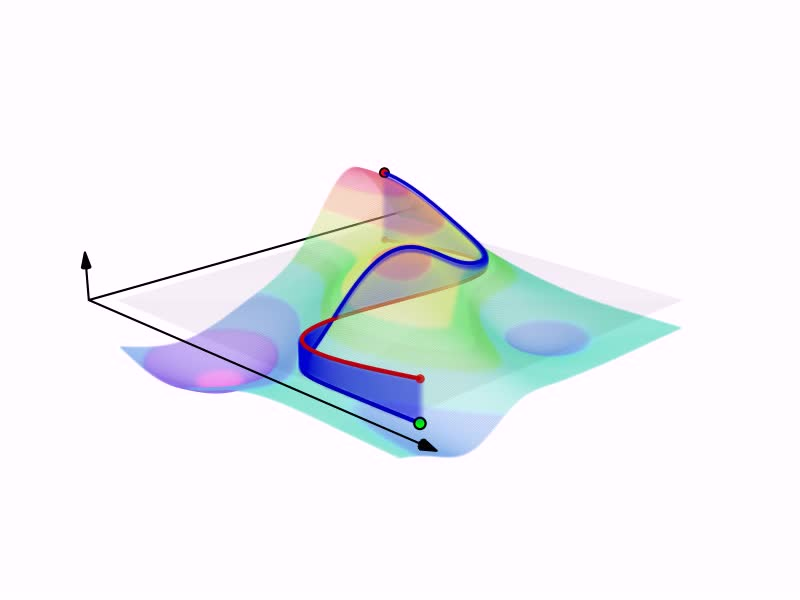
\includegraphics[width=.5\textwidth]{Figures_Part_6/Line_integral_of_scalar_field.jpg}
                       \end{figure}
                       
                       \begin{ex}{Length of a curve}{length_of_curve}
                       Let $f(x,y,z)=1$ and $\curvegamma(t)$ be a curve over $t=a$ to $t=b$.  Then the line integral
                       \[
                       \int_{\curvegamma} fd\curvegamma = \int_a^b \left|\tangentgamma(t)\right|dt
                       \]
                      which is the length of the curve $\curvegamma$.
                       \end{ex}
                       
                       \begin{ex}{Line Integral on a Paraboloid}{line_int_parabooid}
                       Consider the function $f(x,y)=x^2+y^2$ and $\curvegamma(t)=\begin{pmatrix} t \\ t \end{pmatrix}$ over $t=0$ to $t=1$.  Then the line integral
                       \[
                       \int_{\curvegamma} fd\curvegamma = \int_0^1 f(\curvegamma(t))\left|\tangentgamma(t)\right|dt.
                       \]
                       We have
                       \begin{itemize}
                           \item $f(\curvegamma(t))=t^2+t^2=2t^2.$
                           \item $\left|\tangentgamma(t)\right|=\left|\begin{pmatrix} 1 \\ 1\end{pmatrix}\right|=\sqrt{2}.$
                       \end{itemize}
                       So we have
                       \[
                       \int_{\curvegamma} fd\curvegamma = \int_0^1 2\sqrt{2}t^2dt.
                       \]
                       This evaluates to $\frac{2\sqrt{2}}{3}$.
                       \end{ex}
                       
                       \begin{exercise}
                       Integrate $f(x,y)=x+y$ along the curve $\curvegamma(t)=\begin{pmatrix} t \\ 0 \end{pmatrix}$ from $t=0$ to $t=1$. What do you notice about this? Can we tie this to one-dimensional integration?
                       \end{exercise}
                       
                      
                       
        
        

